% $Header: /cvsroot/latex-beamer/latex-beamer/solutions/generic-talks/generic-ornate-15min-45min.en.tex,v 1.5 2007/01/28 20:48:23 tantau Exp $

\documentclass{beamer}

% This file is a solution template for:

% - Giving a talk on some subject.
% - The talk is between 15min and 45min long.
% - Style is ornate.



% Copyright 2004 by Till Tantau <tantau@users.sourceforge.net>.
%
% In principle, this file can be redistributed and/or modified under
% the terms of the GNU Public License, version 2.
%
% However, this file is supposed to be a template to be modified
% for your own needs. For this reason, if you use this file as a
% template and not specifically distribute it as part of a another
% package/program, I grant the extra permission to freely copy and
% modify this file as you see fit and even to delete this copyright
% notice. 


\mode<presentation>
{
  \usetheme{Warsaw}
  % or ...

  \setbeamercovered{transparent}
  % or whatever (possibly just delete it)
}


\usepackage[spanish,english]{babel}
% or whatever

%\usepackage[latin1]{inputenc}
\usepackage[utf8]{inputenc}
% or whatever

\usepackage{times}
\usepackage[T1]{fontenc}
% Or whatever. Note that the encoding and the font should match. If T1
% does not look nice, try deleting the line with the fontenc.

\usepackage{amsmath}
\usepackage{eurosym}  
\usepackage{graphicx} 
\usepackage{float}
\usepackage{booktabs}
\usepackage{multicol}

% path to directories containing images
\graphicspath{{./logos/}{./figures/}{./diagrams/}} % Edit this to your
                                % needs. Only logos is really required
                                % when you generate your own content.


\title[Manual de referencia para el desarrollo de robots de Eurobot] % (optional, use only with long paper titles)
{Manual de referencia para el desarrollo de robots de Eurobot}

\subtitle
{Trabajo Fin de Carrera} % (optional)

\author[Javier Baliñas Santos] % (optional, use only with lots of authors)
{
	Javier Baliñas Santos\\ 
	Director: Julio Pastor Mendoza
}
% - Use the \inst{?} command only if the authors have different
%   affiliation.

\institute[Universities of Somewhere and Elsewhere] % (optional, but mostly needed)
{
	\textsc{Departamento de Electrónica}\\
	\vspace{.5cm} 
	\includegraphics[height=1cm]{logoUAHazul}\\ 
	\textsc{Universidad de Alcalá}
}
% - Use the \inst command only if there are several affiliations.
% - Keep it simple, no one is interested in your street address.

\date[29 de septiembre de 2016] % (optional)
{29 de septiembre de 2016}

\subject{Talks}
% This is only inserted into the PDF information catalog. Can be left
% out. 

% If you have a file called "university-logo-filename.xxx", where xxx
% is a graphic format that can be processed by latex or pdflatex,
% resp., then you can add a logo as follows:

% \pgfdeclareimage[height=0.5cm]{university-logo}{university-logo-filename}
% \logo{\pgfuseimage{university-logo}}



% Delete this, if you do not want the table of contents to pop up at
% the beginning of each subsection:
%\AtBeginSubsection[]
%{
%  \begin{frame}<beamer>{Cont}
%    \tableofcontents[currentsection,currentsubsection]
%  \end{frame}
%}

\AtBeginSection[]
{
  \begin{frame}<beamer>
    %\frametitle{Contenido} 
    %\setcounter{tocdepth}{2}
    \tableofcontents[currentsection]
  \end{frame}
}


% If you wish to uncover everything in a step-wise fashion, uncomment
% the following command: 

%\beamerdefaultoverlayspecification{<+->}


\begin{document}

\begin{frame}
  \titlepage
\end{frame}

\begin{frame}{Contenido}
	\setcounter{tocdepth}{1}
	\tableofcontents%[pausesections]
  	% You might wish to add the option [pausesections]
\end{frame}


% Since this a solution template for a generic talk, very little can
% be said about how it should be structured. However, the talk length
% of between 15min and 45min and the theme suggest that you stick to
% the following rules:  

% - Exactly two or three sections (other than the summary).
% - At *most* three subsections per section.
% - Talk about 30s to 2min per frame. So there should be between about
%   15 and 30 frames, all told.

%\section{Example}

%\subsection[Short First Subsection Name]{First Subsection Name}

%\begin{frame}{Make Titles Informative. Use Uppercase Letters.}{Subtitles are optional.}
%  % - A title should summarize the slide in an understandable fashion
%  %   for anyone how does not follow everything on the slide itself.

%  \begin{itemize}
%  \item
%    Use \texttt{itemize} a lot.
%  \item
%    Use very short sentences or short phrases.
%  \end{itemize}
%\end{frame}

%\begin{frame}{Make Titles Informative.}

%  You can create overlays\dots
%  \begin{itemize}
%  \item using the \texttt{pause} command:
%    \begin{itemize}
%    \item
%      First item.
%      \pause
%    \item    
%      Second item.
%    \end{itemize}
%  \item
%    using overlay specifications:
%    \begin{itemize}
%    \item<3->
%      First item.
%    \item<4->
%      Second item.
%    \end{itemize}
%  \item
%    using the general \texttt{uncover} command:
%    \begin{itemize}
%      \uncover<5->{\item
%        First item.}
%      \uncover<6->{\item
%        Second item.}
%    \end{itemize}
%  \end{itemize}
%\end{frame}


\section{Introducción}

\begin{frame}{La competición Eurobot}
\begin{center}
\alt<1>{
\includegraphics[width=.6\textwidth]{eurobot2}}{}
\alt<2>{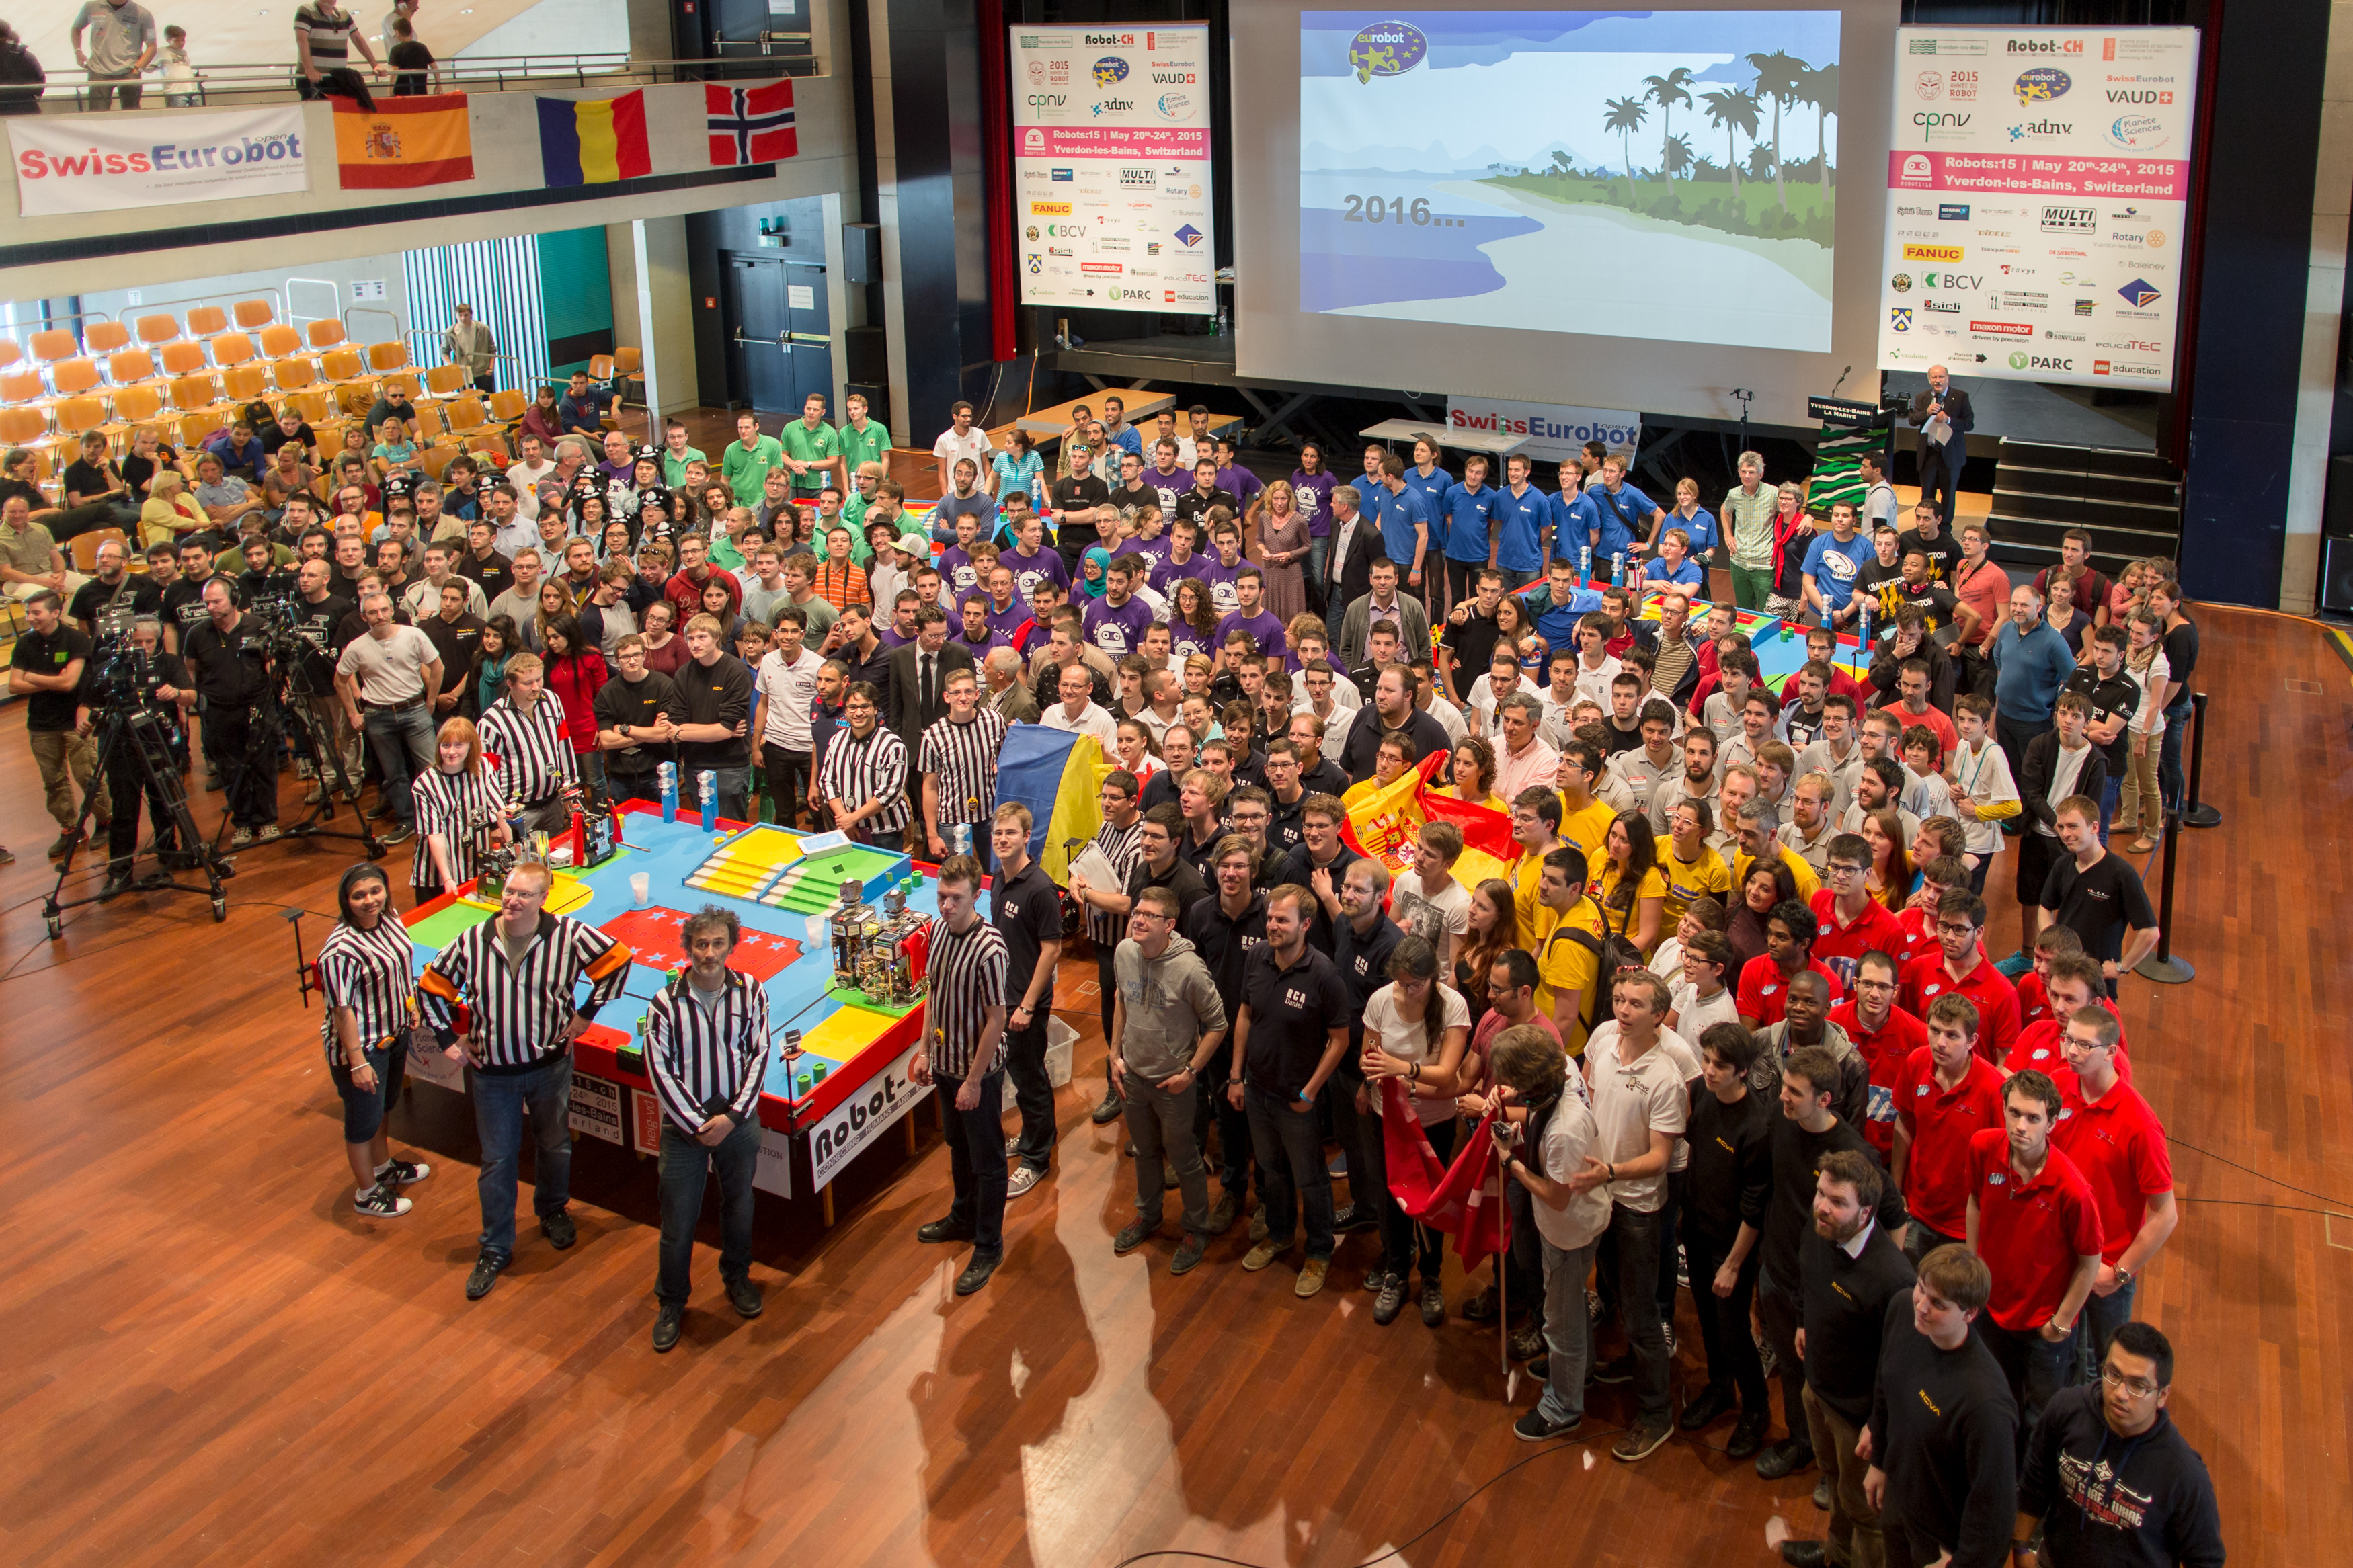
\includegraphics[width=.9\textwidth]{eurobot_family}}{}
\end{center}
\end{frame}

\begin{frame}{Eurobotics Engineering}

\begin{columns}
\column{.5\textwidth}
\centering

\includegraphics[width=\textwidth]{bombona}

\column{.5\textwidth}
\centering
\alt<1>{
\includegraphics[width=\textwidth]{arc_logo_cartel}\\
		
\includegraphics[width=\textwidth]{logotexto1}}{}

\alt<2>{
\includegraphics[width=\textwidth]{Logo_depeca_Grande_rojo_2_150ppp}}{}

\alt<3>{
\includegraphics[width=\textwidth]{AYTO-COSLADA}\\
		
\includegraphics[width=\textwidth]{ayudas_hidraulicas}\\
		\vspace{.2cm}
		
\includegraphics[width=.7\textwidth]{splashscreen_logo}}{}

\end{columns}
\end{frame}

\begin{frame}{Motivación}

\begin{itemize}
\item Afición a la robótica, electrónica y los sistemas embebidos
\item Inquietud Maker
\item Divulgación del conocimiento
\end{itemize}

\end{frame}


\section{El robot de Eurobot}
\subsection{Especificaciones}

\begin{frame}{El juego y sus elementos}
\includegraphics[width=.9\textwidth]{campo_2015}
\end{frame}

\begin{frame}{Los robots}
\begin{columns}
\column{.5\textwidth}

\begin{itemize}
\item Autónomo (90s)
\item Realizar acciones del juego
\item Evitar colisiones
\item Hasta 2 robots por equipo
\item Perímetro máximo 1,2/1,5m (70/90cm)
\item Altura máxima 35cm
\item Balizas campo y robot oponente
\end{itemize}

\column{.5\textwidth}
\centering
\includegraphics[width=\textwidth]{balizas_robots}
\end{columns}
\end{frame}


\subsection{Funcionalidades}

\begin{frame}{Funcionalidades a desarrollar}

\begin{enumerate}
\item<4-> Estrategia de juego
\item<1-> Desplazamiento y localización
\item<2-> Evitación de obstáculos
\item<5-> Comunicación entre robots
\item<3-> Manipulación de elementos de juego
\end{enumerate}

\end{frame}

\begin{frame}{La plataforma robótica base}
\centering
\includegraphics[width=.9\textwidth]{partes_robot_eurobot}
\end{frame}

\subsection{Desarrollo}

\begin{frame}{Fases de desarrollo}

\begin{itemize}
\item<1-> Fabricación del campo de juego y sus elementos
\item<2-> Diseño de la estrategia
\item<3-> Realización de prototipos mecánico y pruebas de concepto
\item<4-> Diseño y fabricación de la mecánica y de la electrónica
\item<5-> Montaje del robot y cableado
\item<4-> Implementación SW de la funcionalidad del robot
\item<4-> Implementación SW de la estrategia de juego
\item<6-> Puesta en marcha y verificación
\end{itemize}
\end{frame}

\section{Plataforma robótica base}
\subsection{Partes principales}

\begin{frame}{Bloque motor y electrónica}
\begin{center}
\alt<1>{\includegraphics[height=.8\textheight]{plataforma_partes_1}}{}
\alt<2>{\includegraphics[height=.8\textheight]{sistema_traccion_rollones}}{}
\end{center}
\end{frame}

\begin{frame}{Ruedas libres}
\begin{center}
\alt<1>{\includegraphics[width=\textwidth]{ruedas_libres_lineal}}{}
\alt<2>{\includegraphics[width=\textwidth]{ruedas_libres_pivotante}}{}
\end{center}
\end{frame}

\begin{frame}{Detección de obstáculos y oponentes}
\begin{center}
\alt<1>{\includegraphics[height=.8\textheight]{plataforma_partes_2}}{}
\end{center}
\end{frame}

\subsection{Dinámica}

\begin{frame}{Desplazamiento lineal sobre un plano horizontal}
\end{frame}

\begin{frame}{Coheficiente de adherencia $K_a$}
\begin{center}
\alt<1>{\includegraphics[width=.9\textwidth]{dinamica_basica}\\

		\begin{equation*}
		  \label{eq_fx_max_f_ka}
		  F_{x\,max} = K_a \, F_n
		\end{equation*}
}{}

\alt<2>{\includegraphics[width=.8\textwidth]{metodo_cubo}\\

		\begin{equation*}
		  \label{eq_ka=f(p1,p2)}
		  \boxed{K_a = \frac{P2}{P1}}
		\end{equation*}
}{}

\alt<3>{\includegraphics[width=.4\textwidth]{ruedas_foam_silicona}\\
		\vspace{.5cm}
		\begin{tabular}{lccc}
		\hline
		Robot & $P1$ & $P2$ & $K_a$ \\
		\hline
		Zamorano (2011) 	& 14,5   & 15,6   & 1,076  \\
		Automático (2012)   & 17,6   & 17,3   & 0,983  \\
		\hline
		\end{tabular}
}{}
\end{center}
\end{frame}

\begin{frame}{Aceleración máxima de un robot con ruedas atrás}
\begin{center}
\alt<1>{\includegraphics[width=.4\textwidth]{dinamica_a_max_ruedas_atras}\\
		\vspace{.2cm}
		\includegraphics[width=.8\textwidth]{dinamica_a_max_ruedas_medio}
}{}

\alt<2>{\includegraphics[width=.4\textwidth]{dinamica_a_max_ruedas_atras}\\

		\begin{align*}
		(2F1)/mg &= d2/d + (a/g)(h/d)\\
		(2F2)/mg &= d1/d - (a/g)(h/d)
		\end{align*}
}{}

\alt<3>{
\begin{columns}
\column{.5\textwidth}
\includegraphics[width=.8\textwidth]{dinamica_a_max_ruedas_atras}\\
Condición de derrape:
\begin{equation*}
|F_x| < K_a \, F1.
\end{equation*}

Condición de \emph{caballito}:
\begin{equation*}
F2 > 0, F1 > 0
\end{equation*}

\column{.5\textwidth}
Fase de aceleración ($a>0$):
\begin{align*}
a_{max1} &= g\,\frac{K_a \, d2}{d-(K_a \, h)}\\
a_{max2} &= g\,\frac{d1}{h}
\end{align*}

Fase de frenado ($a<0$):
\begin{align*}
a_{max1} &= g\,\frac{K_a \, d2}{d+(K_a \, h)}\\
a_{max2} &= g\,\frac{d2}{h}
\end{align*}

%\begin{equation*}
%a_{max} = Min\{a_{max1}, a_{max2}\}
%\end{equation*}
\end{columns}
}{}

\alt<4>{\includegraphics[width=.9\textwidth]{ejemplo_a_max}\\
		\vspace{.3cm}
	
		\begin{tabular}{ lcccc }
		\hline
					& Acel. R1 & Fren. R1 & Acel. R2 & Fren. R2 \\
		\hline
		$a_{max1}$ 	& $1,2g$ 		& $0,4g$ 		& $3,0g$ 		& $0,3g$ 	\\
		$a_{max2}$ 	& $0,8g$ 		& $1,2g$ 		& $0,5g$ 		& $0,75g$ 	\\
		$a_{max}$ 	& $0,8g$ 		& $0,4g$ 		& $0,5g$ 		& $0,3g$ 	\\
					& ($8\,m/s$) 		& ($4\,m/s$) 		& ($5\,m/s$) 		& ($3\,m/s$)  \\
		\hline
		\end{tabular}
}{}

\alt<5>{\includegraphics[width=.6\textwidth]{medida_centro_gravedad}\\
}{}

\end{center}
\end{frame}

\begin{frame}{Perfil de velocidad trapezoidal}
\begin{center}
\includegraphics[width=.55\textwidth]{perfil_trapezoidal}
\end{center}
\end{frame}

\begin{frame}{Dimensionamiento de la reductora}
\begin{center}
\alt<1>{\includegraphics[width=.9\textwidth]{modelo_reductora_motor}\\
		\vspace{.5cm}
		\begin{columns}
		\column{.5\textwidth}
		El par en el motor necesario:
		\begin{equation*}
		M1 = \frac{K_a\,mg\,(d2/d)}{K\,Rd\,D}
		\end{equation*}

		\column{.5\textwidth}
		Par motor máximo en la reductora:
		\begin{align*}
		M2 &= K_m\,i = K_m\,\frac{v_{sat}}{r}
		\end{align*}
		\end{columns}
}{}

\alt<2>{\includegraphics[width=.9\textwidth]{modelo_reductora_motor}\\
		\vspace{.5cm}
		\begin{columns}
		\column{.5\textwidth}
		Condición de deslizamiento:
		\begin{equation*}
		M2 >= 1,2\,M1
		\end{equation*}

		\column{.5\textwidth}
		Valor de reducción:
		\begin{equation*}
		\boxed{K_{min} = 1,2\,\frac{K_a\,mg\,(d2/d)\,D\,r}{4\,K_m\,Rd\,v_{sat}}}
		\end{equation*}
		\end{columns}
}{}

\end{center}

\end{frame}

\begin{frame}{Velocidad máxima}
\end{frame}


\subsection{Control de posición polar}

\begin{frame}{Controladores de ángulo y distancia}
\end{frame}

\begin{frame}{Implementación del perfil trapezoidal}
\end{frame}

\begin{frame}{Ajuste de los controladores}
\end{frame}

\subsection{Odometría}

\begin{frame}{Calculo de la posición del robot}
\end{frame}

\begin{frame}{Medida y corrección de errores sitemáticos}
\end{frame}


\subsection{Baliza tipo faro}

\begin{frame}{Mecánica de la baliza}
\begin{center}
\alt<1>{\includegraphics[width=.9\textwidth]{baliza_mecanica}}{}
\alt<2>{\includegraphics[width=.8\textwidth]{baliza_catadioptrica}}{}
\end{center}
\end{frame}

\begin{frame}{Fundamento}
\begin{center}
\alt<1>{\includegraphics[height=.9\textheight]{baliza_fundamento}}{}
\end{center}

\alt<2>{\includegraphics[width=\textwidth]{baliza_signal}}{}
\end{frame}

\begin{frame}{Implementación y resultados}
\alt<1>{\includegraphics[height=.8\textheight]{baliza_bloques_hw_sw}}{}
\begin{center}
\alt<2>{\includegraphics[height=.8\textheight]{beacon_robot_calib_3m_fig_1_small.pdf}}{}
\end{center}
\end{frame}


\section{Desarrollo HW y SW}

\appendix
\section*{Conclusiones}

\begin{frame}{Conclusiones}

  % Keep the summary *very short*.
  \begin{itemize}
  \item
    The \alert{first main message} of your talk in one or two lines.
  \item
    The \alert{second main message} of your talk in one or two lines.
  \item
    Perhaps a \alert{third message}, but not more than that.
  \end{itemize}
  
  % The following outlook is optional.
  \vskip0pt plus.5fill
  \begin{itemize}
  \item
    Outlook
    \begin{itemize}
    \item
      Something you haven't solved.
    \item
      Something else you haven't solved.
    \end{itemize}
  \end{itemize}
\end{frame}


\end{document}


